\chapter{Identifikation von Datenassoziationen zum Karten-Update}\label{chapter:association}

Wie in der Einleitung beschrieben, soll in einem ersten Ansatz analysiert werden, ob eine TSDF Karte mit gegebenem initialen Pfad durch dessen Optimierung mittels Schleifenschlüssen verbessert werden kann. Dazu ist im ersten Schritt zu identifizierten, welcher Teil der Karte mit welcher Pose assoziiert ist, um bei einer Veränderung der Trajektorie entscheiden zu können, wie die Karte angepasst werden muss. Dies Kapitel befasst sich mit der Generation von Datenassoziationen zwischen den Posen des Pfades und der TSDF-Karte.

\section{Ansatz}
\label{section:ansatz}

Wie in Kapitel \ref{section:tsdf} beschrieben, wird die TSDF Karte von Eisoldt et al. \cite{HATSDF} inkrementell erweitert, sobald eine definierte minimale Distanz zurückgelegt wurde. Dabei werden nicht nur neue Zellen beschrieben, sondern auch die Werte bereits beschriebener Zellen gewichtet verändert. Dementsprechend kann die Information in einer Zelle eine Akkumulation beliebig vieler Updates sein und beliebig vielen Posen zugeordnet werden. Diese Information gilt es zu berücksichtigen, wenn auf Basis einer gegebenen TSDF Karte Datenassoziationen identifiziert werden sollen.
Eine Möglichkeit der Generation dieser Assoziation wäre eine \emph{1:1} Beziehung zwischen den Zellen und Posen aufzubauen. Dann würde eine Zelle maximal einer Pose zugeordnet werden. Da bereits bekannt ist, dass eine Zelle von mehreren Posen angepasst werden kann, ist diese Art der Beziehung zwischen Posen und TSDF-Zellen allerdings von einem großen Informationsverlust geprägt. Die Alternative zur \emph{1:1} Beziehung ist eine \emph{1:N} Beziehung zwischen einer Zelle und $N$ Posen. Diese Beziehung ist aufgrund der genannten Eigenschaften des TSDF-Karten Updates der \emph{1:1} Beziehung zu bevorzugen.

Die Informationen darüber, welche Position welche TSDF Zelle beschrieben hat, lässt sich allerdings nicht aus der TSDF Karte herauslesen. Um dies zu ermöglichen könnte der Ansatz von Eisoldt et al. \cite{HATSDF} um die Funktion erweitert werden, an jeder Zelle zusätzlich ein Array zu speichern, in dem die Posen enthalten sind, die die betroffene Zelle modifiziert haben. Dieses Array muss in einem eigenen Datensatz gespeichert sein, da die Anzahl Posen, die auf diese Weise einer Zelle zugeordnet werden können, dynamisch ist. Das bedeutet, dass für jede einzelne TSDF Zelle ein eigenes Datensatz gespeichert werden muss, in dem die zugehörigen Posen enthalten sind. Je nach Auflösung der diskretisierten Karte müssten nach diesem Ansatz mehrere Millionen separate Datensätze gespeichert werden. Ein solches Vorgehen erfordert nicht nur viel Speicher, sondern ist auch aus hierarchischer Betrachtungsweise keine sinnvolle Herangehensweise.
Eine Möglichkeit, die gewünschten Daten auf Basis einer gegebenen TSDF Karte zu generieren ist diese über die Methode, mit der die Daten generiert wurden, zu regenerieren. In \cite{HATSDF} wird die TSDF-Karte über ein \emph{Ray-Marching} generiert. Eine alternative zum Ray-Marching stellt der Bresenham- Algorithmus \cite{bresenham1965algorithm} dar, der die Diskretisierung der Karte ausnutzt.
Beide Varianten werden im Folgenden beschrieben, evaluiert und miteinander verglichen.
Zunächst beschreibt der folgende Abschnitt die Serialisierung der Datenassoziation in der HDF5-Datenstruktur.

\section{Serialisierung der Datenassoziationen}


Dieser Abschnitt beschreibt, wie identifizierte Assoziationen in der hierarchischen Struktur der HDF5-Datei gespeichert werden, die Daten der TSDF-Karte, sowie die zugehörige Pose-Historie enthält.
Wie in Kapitel \ref{section:tsdf} beschrieben, enthält die HDF5 Struktur mehrere Gruppen, die jeweils weitere Daten enthalten. Zu diesen Gruppen gehören in diesem Fall \textit{/map} und \textit{/poses}.
Die Map-Gruppe enthält die serialisierten TSDF-Zellenwerte und TSDF-Zellengewichte. Die Poses-Gruppe enthält die serialisierten 6D Posen des Pfades als Datensätze.
Der HDF5 interne Pfad eines dieser Pose-Datensätze ist \textit{/poses/[index]}, wobei \textit{index}, der Index der Pose im Pfad ist.
An dieser Stelle wird nun einer Erweiterung vorgenommen, um die generierten Assoziationen zu serialisieren. Anstelle der Datensätze wird für jede Pose eine eigene Gruppe erstellt. Diese Gruppe erhält als Namen ebenfalls den Pfadindex der Pose. Innerhalb dieser Gruppe wird ein Datensatz für die Pose und optional ein weiteres Datensatz für die Datenassoziationen angelegt, sofern erforderlich.
Abbildung \ref{fig:hdf5new} zeigt die neue interne HDF5 Struktur nach dieser Änderung.

\begin{figure}
		\centering
		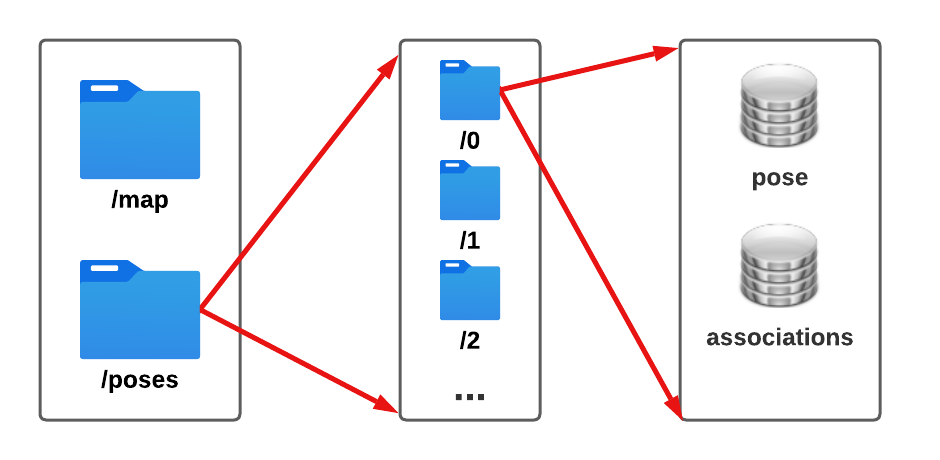
\includegraphics
			[scale=0.4]
			{HDF5new}
		\caption
			[Caption for LOF]{Schematische Darstellung der HDF5 internen Datenstruktur nach Speicherung der generierten Datenassoziationen zwischen TSDF-Zellen und Posen. Die in Kapitel \ref{section:ansatz} beschrieben \textit{1:N} Beziehung zwischen einer Zelle und den zugehörigen Posen ist hier indirekt realisiert. Anstelle pro Zelle ein Datensatz zu erstellen, wir für jede Pose ein Datensatz enthält, das alle assoziierten TSDF-Zellen enthält. Verschiedene Posen können dabei dieselbe TSDF-Zelle assoziieren. Das Datensatz \textit{pose} enthält die Transformation der aktuellen Pose ins Ursprungskoordinatensystem. Das Datensatz \textit{associations} enthält ein Array der assoziierten Zellkoordinaten, die durch die Diskretisierung ganzzahlig sind und als Integer abgespeichert werden.}			                                                                                                                                     
		\label{fig:hdf5new}
\end{figure}

Auf Basis dieser Änderungen wird im Folgenden erläutert, wie die zu speichernden Zellen für jede Pose ermittelt werden.

\section{Detektions-Algorithmen}

Dieser Abschnitt stellt die Algorithmen heraus, mit denen beschriebene Assoziationen identifiziert werden können. Die Ergebnisse der Algorithmen werden miteiander verglichen und evaluiert.

\subsection{Ray-Tracing}
\label{section:ray-tracing}

Eine Möglichkeit der Ermittlung der mit einzelnen Posen assoziierten Teilbereiche der TSDF Karte ist die die Erstellung eines künstlichen Laserscans innerhalb der TSDF Karte, ausgehend von der entsprechenden Pose. Entsprechend wurde im Zuge dieser Arbeit ein \emph{Raytracer} entwickelt, der simulierte Laserstrahlen ausgehend von einer definierten 6D-Pose generiert und die Schnittpunkte der Strahlen mit der TSDF Karte überprüft. Der Raytracer ist beliebig konfigurierbar und kann an die Parameter verschiedenster realer Laserscanner angepasst werden. Die wesentlichen Parameter und deren Bedeutung sind Tabelle \ref{table:Raytracer_params} zu entnehmen.
	
	\begin{table}
		\centering
		\caption{Parameter des in dieser Arbeit entwickelten Raytracers zur Bestimmung des mit einer beliebigen Pose assoziierten Teilbereichs der TSDF-Karte. Der horizontale Öffnungswinkel wird an dieser Stelle als $360$ Grad angenommen.}
		\begin{tabular}{| p{3cm} | p{8cm} | p{2cm} |}
			\hline
			\thead{Parameter}   & \thead{Funktionsweise}  & \thead{Default-\\Wert}\\
			\hline
			$opening\_degree$   & Definiert den vertikalen Öffnungswinkel des Raytracers. Anzugeben in Grad. & $45$ \\
			\hline
			$hor\_res$     & Definiert die horizontale Auflösung des Laserscanners. Der gegebene Wert  entspricht der Anzahl Strahlen pro Scanebene. & $1024$\\
			\hline			
			$vert\_res$    & Definiert die vertikale Auflösung des Laserscanners. Der gegebene Wert entspricht der Anzahl an Scanebenen im Laserscan. & $128$\\
			\hline			
			$step\_size$      & Definiert, wie groß die Schrittweite beim Aussenden der einzelnen Strahlen ist. Der Wert ist in Metern anzugeben. Der Default-Wert ist direkt an die Zellgröße der diskreten TSDF-Karte $map_{res}$ gekoppelt und beträgt $\frac{map_{res}}{2}$. & $0.032$ \\
			\hline			
			$ray\_size$   & Definiert die Dicke des Strahls in der Visualisierung. Dieser Parameter dient lediglich zur erleichterten Visualisierung des Laserscans bei unterschiedlicher Konfiguration. Der Wert ist in Metern anzugeben. & $0.01$ \\
			\hline
		\end{tabular}
		\label{table:Raytracer_params}
	\end{table}	
	
Zur Emulation das Laserscans wird zunächst ein Array erstellt, in dem die aktuellen Endpunkte der jeweiligen Strahlen gespeichert werden. Die Anzahl an Endpunkten $n$ ist definiert durch die konfigurierte Auflösung. Sie beträgt:

\begin{myequation}
n = \text{vert\_res} \cdot \text{hor\_res}
\end{myequation}

 Der Startpunkt jedes Strahls ist die Pose $P_i$, von der aus der Laserscan ausgesendet wird. Ziel ist in jeder Iteration alle Strahlen um $step\_size$ zu verlängern und die TSDF-Zellen zu evaluieren, die derzeit von den einzelnen Strahlen getroffen werden. Für diese Verlängerung der Strahlen müssen diese zunächst initialisiert werden. Diese Initialisierung erfolgt auf Basis der parametrisierten Öffnungswinkel des Laserscanners $opening\_degree\_vert$ und $opening\_degree\_hor$, sowie der konfigurierten vertikalen und horizontalen Auflösung $vert\_res$ und $hor\_res$.
Zunächst werden die Winkelbereiche definiert, in den der Raytracer operiert. Diese setzten sich aus den Öffnungswinkeln zusammen. Der Winkelbereich in horizontaler Richtung beträgt:

\begin{myequation}
I_{hor} = \left[-\text{opening\_degree\_hor}, \text{opening\_degree\_hor} \right]
\end{myequation}

Der Winkelbereich in vertikaler Richtung beträgt:

\begin{myequation}
I_{vert} = \left[-\text{opening\_degree\_vert}, \text{opening\_degree\_vert} \right]
\end{myequation}

Die jeweiligen Winkelbereiche werden durch die konfigurierte Auflösung diskretisiert.
Die horizontale Schrittweite des Laserscanners beträgt:

\begin{myequation}
\Delta_{hor} = \frac{opening\_degree\_hor}{hor\_res}
\end{myequation}

Die vertikale Schrittweite des Laserscanners beträgt:

\begin{myequation}
\Delta_{vert} = \frac{opening\_degree\_vert}{vert\_res}
\end{myequation}

Basierend auf den unteren und oberen Winkelschranken und der berechneten Schrittweite zwischen diesen Schranken kann nun das Array initialisiert werden. Dazu wird in zwei Schleifen über die beiden Winkelintervalle $I_{vert}$ und $I_{hor}$ iteriert und der aktuelle Wert jeweils um die berechneten Delta $\Delta_{vert}$ und  $\Delta_{hor}$ inkrementiert. Aus den beiden Winkeln $\alpha$ und $\beta$ der aktuellen Iteration der Schleifen, sowie einer beliebigen Distanz initialen Länge des Strahls, wie zum Beispiel der Schrittweite $step\_size$ können nun für jeden Punkt die initialen Ray-Punkte berechnet werden, die den Richtungsvektor des Strahls definieren.
Hierzu ist eine Umwandlung von Kugelkoordinaten in das Kartesische Koordinatensystem notwendig. Mit $alpha$, $beta$ und $step\_size$ wird in Kugelkoordinaten genau ein Punkt im dreidimensionalen Raum beschrieben. Um diese in kartesische Koordinaten im ROS Koordinatensystem umzuwandeln wird folgende Formel verwendet ($\alpha$ und $\beta$ gegeben in Radianten, $\alpha$ beschreibt den aktuellen Winkel um die z-Achse, $\beta$ die aktuelle Rotation um die y-Achse):

\begin{myequation}
\colvec{x_{P_i}\\y_{P_i}\\z_{P_i}} = \text{step\_size} \cdot \colvec{\cos\left(\alpha \right) \cdot \cos\left(\beta \right) \\ \sin\left(\alpha \right) \cdot \cos\left(\beta \right) \\ \sin\left(\beta \right)}
\end{myequation}

Der Punkt $\left(x_{P_i}, y_{P_i}, z_{P_i} \right)^T$ beschreibt hier zunächst nur den Startpunkt des Strahls aus Sicht des lokalen Karten-Koordinatensystems, das durch ${P_i}$ beschrieben ist. Um diesen aus Sicht des globalen Koordinatensystems $\mathbb{M}$ zu betrachten, muss dieser Punkt dorthin transformiert werden. Grundlagen zur Transformation werden in Kapitel \ref{section:transformationen} behandelt. Es ist essentiell, dass an dieser Stelle nicht nur die Translation, sondern auch die Rotation berücksichtigt wird um den Scan von Pose $P_i$ bestmöglich replizieren zu können. Die Transformation des Vektors $\left( x_{P_i}\\y_{P_i}\\z_{P_i} \right)^T$ vom Koordinatensystem beschrieben durch Pose $P_I$ in das globale Koordinatensystem $\mathbb{M}$ mit der Transformationsmatrix $T_{P_i \rightarrow \mathbb{M}}$ ist gegeben durch:

\begin{myequation}
\colvec{x_{\mathbb{M}}\\y_{\mathbb{M}}\\z_{\mathbb{M}}} = T_{P_i \rightarrow \mathbb{M}} \cdot \colvec{x_{P_i}\\y_{P_i}\\z_{P_i}}
\end{myequation}

Auf diese Weise werden alle initialen Endpunkte des simulierten Laserscans berechnet. Die Strahlen sind dann jeweils durch den aktuellen Endpunkt und den Startpunkt, der sich aus dem Translationsanteil der Pose $P_i$ ergibt. Dies sorgt dafür, dass die 3-D-Rotationen nur bei der Initialisierung der Strahlen berechnet werden. Im Anschluss kann der berechnete Strahl durch eine Verlängerung des durch den Start- und Endpunkt definierten Vektors abgelaufen werden. In jeder Iteration des Ray-Tracing werden die Vektoren alle Strahlen um $step\_size$ verlängert und die entsprechend getroffenen Zellen evaluiert. Um einen Vektor $\vec{v}$ gegeben durch den Ursprung des Strahls, der sich aus dem  Translationsanteil $\vec{t_i}$ der Pose $P_i$ ergibt und den aktuellen Endpunkt des betrachteten Strahls $\vec{r_i}$ um $step\_size$ zu verlängern und daraus den neuen Endpunkt des Strahls $\hat{\vec{r_{i}}}$ zu berechnen wird folgende Formel verwendet:

\begin{myequation}
\hat{\vec{r_{i}}} = \frac{\norm{\vec{r_i} - \vec{t_i}} + step\_size}{\norm{\vec{r_i} - \vec{t_i}}} \cdot \left( \vec{r_i} - \vec{t_i} \right) + \vec{t_i} 
\end{myequation}

Nach der Verlängerung eines Strahls $\vec{r_i}$ wird die inder aktuellen Iteration $j$ getroffene TSDF-Zelle $C_i^j$ evaluiert. Je nach Schrittweite $step\_size$ und Auflösung des Raytracers ist es möglich, dass $C_i^j$ bereits evaluiert wurde und schon eine Assoziation mit der Pose $P_i$ hergestellt ist. Um diesen Fall zu überprüfen und zu verhindern, dass duplizierte Assoziationen gespeichert werden, wird eine Hash-Map genutzt, deren Hash auf Basis der Koordinaten der TSDF-Zelle berechnet wird. Ist $C_i^j$ bereits in der Hash-Map gespeichert, ist der aktuell betrachtete Strahl $\vec{r_i}$ für diese Iteration evaluiert und der nächste Strahl kann betrachtet werden. Um zu entscheiden, ob eine nicht assoziierte Zelle $C_i^j$ als Assoziation in Frage kommt, müssen mehrere Zustände des Strahls definiert werden. Abbildung \ref{fig:RayTracingBig} zeigt die benötigten Zustände und die Bedinungen für einen Wechsel des Status gegeben den aktuellen Status und die betrachtete Zelle $C_i^j$, sowie dieren TSDF-Wert und TSDF-Gewicht. Ein Strahl ist beschränkt durch die lokale Karte um $P_i$ \ref{section:tsdf_map}, sowie die Struktur der TSDF-Karte. Detektiert ein Strahl einen einen Wechsel von positive auf negative TSDF-Werte (\emph{Nulldurchgang}) in der TSDF, stoppt der Raytracer, sobald er erneut positive Werte detektiert. Diese Herangehensweise sorgt dafür, dass mit der Pose $P_i$ keine Zellen assoziiert werden, die von dieser Pose aufgrund der Begrenzungen der lokalen Karte nicht gesehen werden konnten oder hinter Wänden befindlich sind.

\begin{figure}
		\centering
		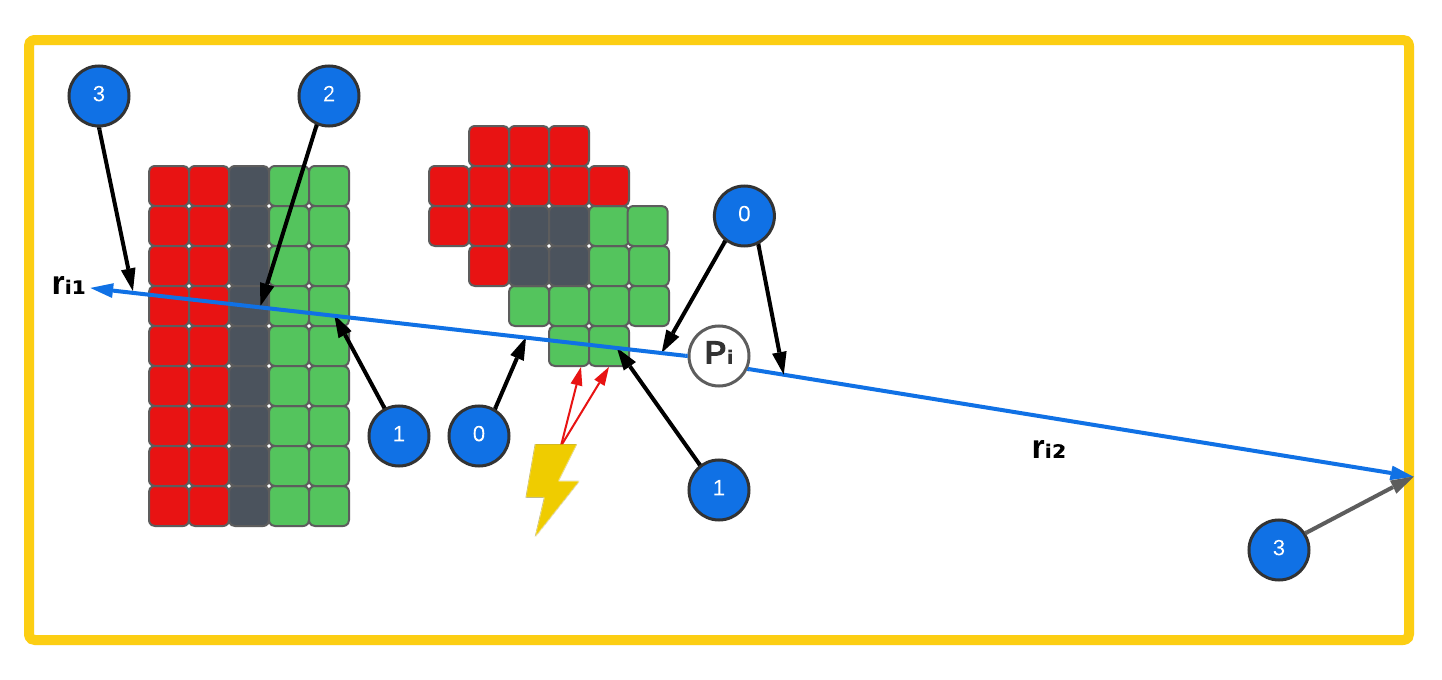
\includegraphics
			[scale=0.3]
			{RayTracingBig}
		\caption
			[Caption for LOF]{Schematische Darstellung 2D Darstellung der verschiedenen Zustände eines einzelnen Strahls des Raytracers innerhalb einer TSDF-Darstellung. Negative TSDF-Werte sind rot dargestellt, positive in grün. Der approximierte Nulldurchgang in der TSDF ist hier gräulich dargestellt, die umgebende lokale Karte in gelb. Ausgehend von Pose $P_i$ sind zwei Strahlen $r_{i1}$ und $r_{i2}$ dargestellt, die die verschiedenen Fälle abdecken, die es zu berücksichtigen gilt. Eine genaue Beschreibung der Zustandsänderungen der Strahlen im Zustandsdisgramm \ref{fig:Ray-Trace-Zustandsdiagramm} zu entnehmen. Die entsprechenden Zustände sind dargestellt als blaue Kreise, die die jeweilige Zustandsnummer enthalten. Die entsprechenden Definitionen der Zustände sind ebenfalls im Zustandsdiagramm \ref{fig:Ray-Trace-Zustandsdiagramm} zu entnehmen. Die mit einem Blitz markierten Zellen werden zwar von dem ausgesandten Strahl $r_{i1}$ getroffen, dürfen allerdings aufgrund der Evidenz im aktuellen Strahl nicht mit der Pose assoziiert werden, da im Anschluss an diese Zellen kein Nulldurchgang, sondern Freiraum folgt. Der Freiraum ist hier in weiß dargestellt und setzt sich aus den TSDF-Zellen zusammen, die Default-Werte enthalten und entsprechend außer der minimalen Entfernung $tau \left(\tau\right)$ zur Oberfläche, keine räumlichen Informationen besitzen. Gleicher Ausnahmefall tritt ein, wenn der Strahl lediglich negative TSDF-Zellen trifft. Diese werden ebenfalls nicht aufgrund der Evidenz des betrachteten Strahls mit der Pose assoziiert.}		                                                                                                                                     
		\label{fig:RayTracingBig}
\end{figure}

\begin{figure}
		\centering
		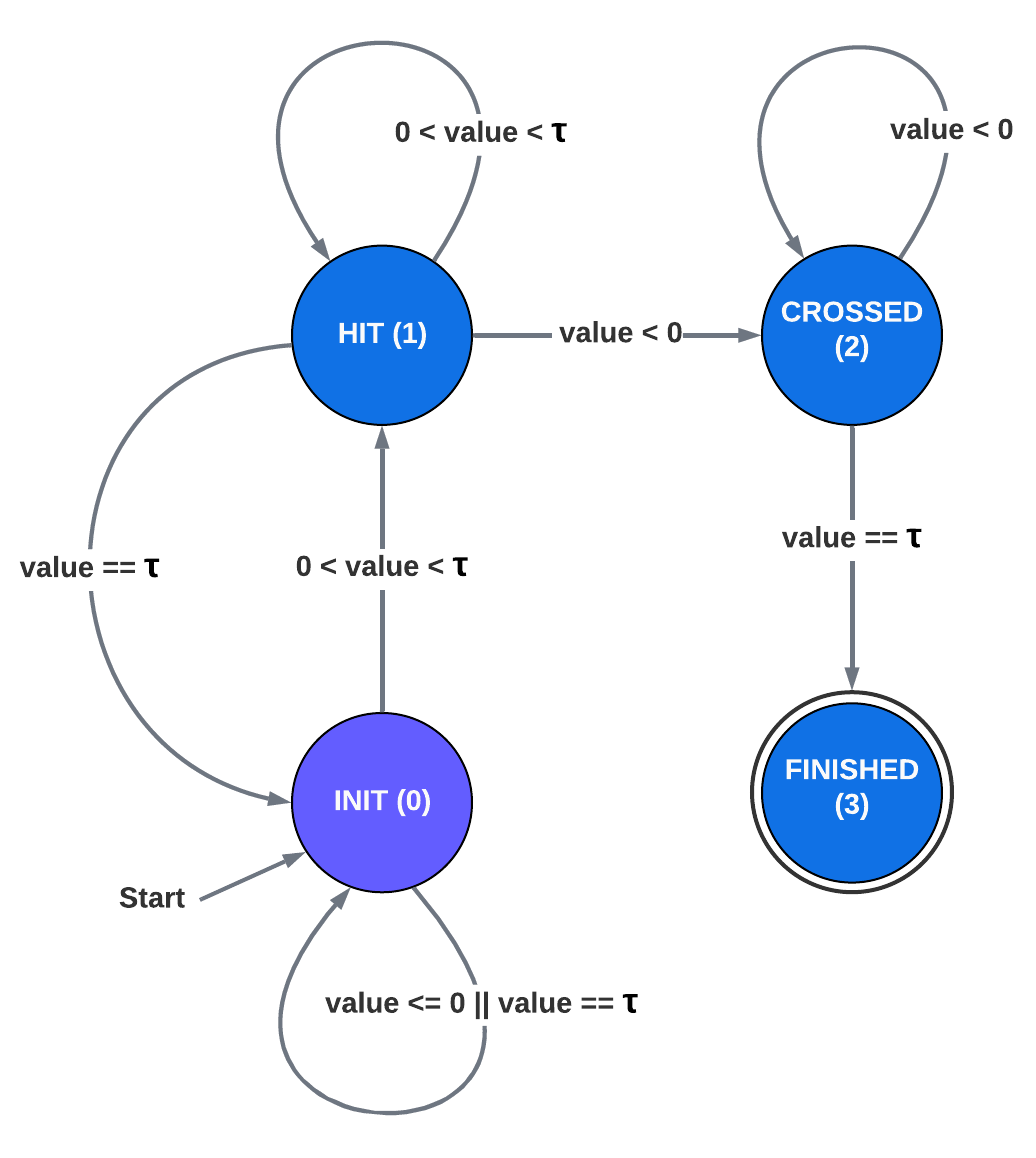
\includegraphics
			[scale=0.25]
			{Ray-Trace-Zustandsdiagramm}
		\caption
			[Caption for LOF]{Zustandsdiagramm der internen Zustände eines Strahls. Zustandsübergänge sind beschrieben durch einen initialen Zustand und den TSDF-Wert der aktuellen Zelle (\textit{value}). In Zustand 1 werden gefundene Assoziationen zunächst nicht abgespeichert, da noch nicht bekannt ist, ob diese Zellen zu einem Nulldurchgang gehören oder ob der Strahl nur Zellen kreuzt, die von einer anderen Pose aus befüllt wurden. Je nach TSDF-Wert der aktuellen Zelle werden die zwischengespeicherten Assoziationen aus Zustand 1 entweder verworfen oder in der HDF5 gespeichert.}		                                                                                                                                     
		\label{fig:Ray-Trace-Zustandsdiagramm}
\end{figure}

Die Ergebnisse dieses Ansatzes sind in Abbildung \ref{fig:bresenham_vs_raytrace} im Vergleich mit den Ergebnisses des Bresenham Algorithmus dargestellt, der im nachfolgenden Abschnitt behandelt wird. In dem genutzten Datensatz können nur etwa $91\%$ der Zellen assoziiert werden. Diese Zahl ähnelt auch der von Bresenham. Bei einer Evaluation weiterer Datensätze ergab sich ebenfalls eine Abdeckung von etwa $90\%$ mit jeweils leicht höherer Abdeckung des Raytracers. Abschnitt \ref{section:association_evaluation} evaluiert die Ergebnisse von Ray-Tracing und Bresenham und vergleicht diese miteinander. Zudem wird Bezug zum Informationsverlust bei der Assoziationsidentifikation genommen.

\subsection{Bresenham}

Eine alternative algorithmische Herangehensweise an das beschriebene Problem der Assoziationsidentifikation ist die Nutzung des Bresenham-Algorithmus \cite{bresenham1965algorithm}. Dieser wurde ursprünglich verwendet, um einen digitalen Plotter mittels eines Computers zu kontrollieren und beliebige zweidimensionale Linien und Kurven approximativ abzubilden. Der Plotter lässt sich dabei in acht Richtungen auf einem diskretisierten Raster bewegen. Bresenham \cite{bresenham1965algorithm} beschreibt, wie sich die Zellen im Raster berechnen lässt, die das gegebene Liniensegment einer Kurve oder eine Linie am besten beschreibt. Der Bresenham Algorithmus findet heutzutage vielfach Anwendung im Bereich der Computergrafik. Hier liegt eine Diskretisierung durch die Auflösung des Bildschirms in Pixeln vor. Mittels des Bresenham Algorithmus kann bestimmt werden, durch welche Pixel eine Linie oder ein Liniensegment beschrieben werden kann. Abbildung \ref{fig:Bresenham2D} zeigt die initiale Idee des Bresenham Algorithmus in 2-D. Eine ähnliche Diskretisierung weist auch die in dieser Arbeit verwendete TSDF-Karte auf. Sie ist allerdings im Gegensatz zu den beschriebenen Beispielen in drei Dimensionen diskretisiert. Mittels Bresenham soll bestimmt werden, welche Voxel der TSDF-Karte zu einem Strahl gehören, der von einer Position $\vec{p}$ ausgesendet wurde und sich mit der TSDF-Karte schneidet. Ziel ist die Beschleunigung des Ray-Tracing Ansatzes durch die Ausnutzung der Diskretisierung der Karte. Dabei gelten die gleichen Voraussetzungen wie beim zuvor beschriebenen Ray-Tracing und die Initialisierung der einzelnen Strahlen erfolgt analog. Im Gegensatz zum Ray-Tracing wird allerdings nicht der Strahl schrittweise verlängert, sondern basierend auf den initialen Richtungsvektoren der Strahlen jeweils das nächste Voxel berechnet, das den Strahl am besten beschreibt.

\begin{figure}
		\centering
		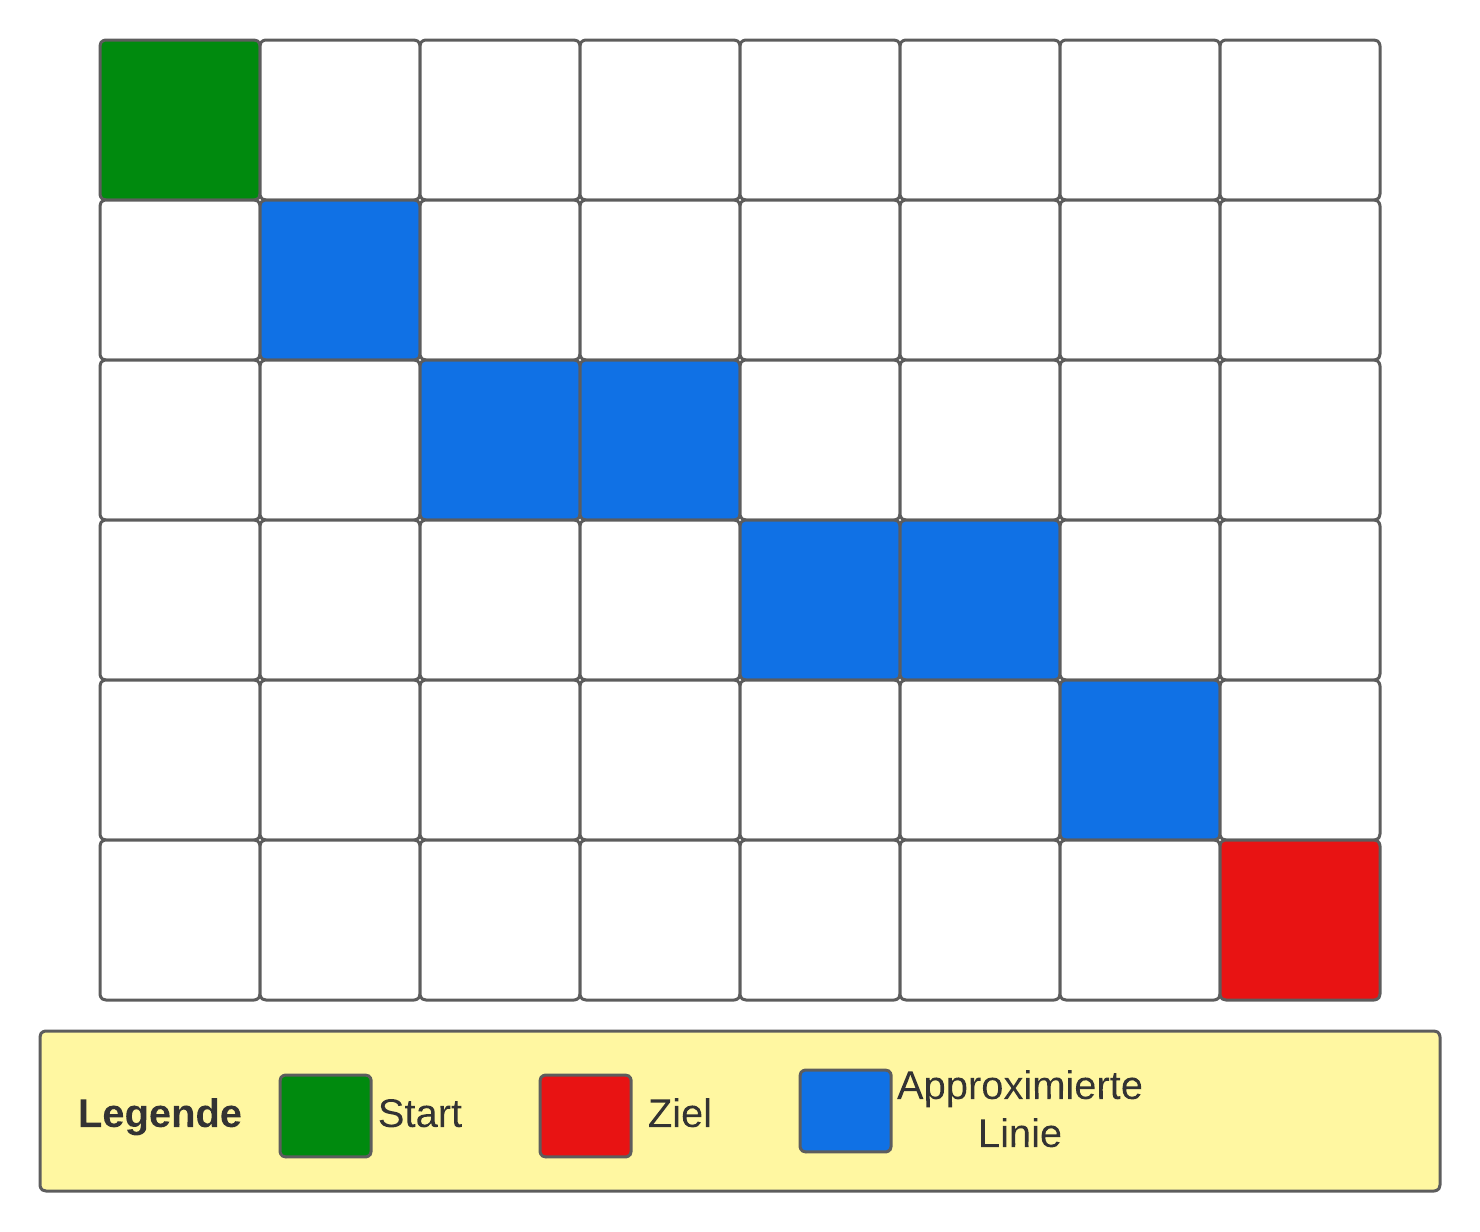
\includegraphics
			[scale=0.2]
			{Bresenham2D}
		\caption
			[Caption for LOF]{Schematische Darstellung des Bresenham-Algorithmus in zwei Dimensionen. Der Bresenham Algorithmus bestimmt, welche Voxel die Linie zwischen einem gegebenen Startvoxel und einem Endvoxel am besten beschreiben.}		                                                                                                                                     
		\label{fig:Bresenham2D}
\end{figure}

Die Grundlage für die Berechnung der zum Strahl gehörigen Voxel bildet ein Startvoxel $\vec{V_{start}}$, gegeben durch die aktuell betrachtete Pose beziehungsweise Scannerposition $P_{i}$ und ein Endvoxel $\vec{V_{end}}$. Letzterer berechnet sich aus dem Schnittpunkt des betrachteten Strahls mit der Bounding-Box der lokalen Karte, gekennzeichnet durch ihren Ursprung $\vec{p_{lmap}}$ und ihre Seitenlängen $\left(s_x, s_y, s_z\right)^T$. Basierend auf den berechneten Start- und Endvoxeln jedes Strahls können nun die dazwischenliegenden Voxel mittels Bresenham ermittelt werden. Der Pseudo-Code in Abbildung \ref{pseudo:bresenham} stellt den Ablauf für die Bestimmung der der Voxel dar, die die Linie gegeben durch den Startvoxel $\vec{V_{start}}$ und Endvoxel $\vec{V_{end}}$ beschreiben. 

\begin{algorithm}
\caption{Bresenham Algorithmus adaptiert in 3D (nach \cite{bresenham1965algorithm})} \label{pseudo:bresenham}
\begin{algorithmic}[1]
\Procedure{Bresenham}{ $\vec{V_{start}}, map_{l}, r_i^j$}
	\State{\emph{\textsl{Initialisierung:}}}
	\State Berechne die Endposition $\vec{V_{end}}$ als Schnittpunkt des Strahls $r_i^j$ mit der lokalen Karte $map_{l}$
	\State Berechne Bresenham Parameter (absolute Abstände und Raumrichtungen):
	\State $dx = \abs{\vec{V_{end}}^x - \vec{V_{start}}^x}$ \Comment{Absolute zwischen den Punkten in alle Raumrichtungen}
	\State $dy = \abs{\vec{V_{end}}^y - \vec{V_{start}}^y}$
	\State $dz = \abs{\vec{V_{end}}^z - \vec{V_{start}}^z}$
	\State $dm = max(dx, dy, dz)$ \Comment Maximale Komponente der Manhattan Distanz
	\State $sx = \vec{V_{start}}^x < \vec{V_{end}}^x$ ? $1$ : $-1$ \Comment{Raumrichtung}
	\State $sy = \vec{V_{start}}^y < \vec{V_{end}}^y$ ? $1$ : $-1$
	\State $sz = \vec{V_{start}}^z < \vec{V_{end}}^z$ ? $1$ : $-1$
	\State \textbf{\textsl{Temporäre Vektoren zur Iteration initialisieren:}} 
	\State $\vec{v_0} = \left(x_0, y_0, z_0\right)^T = \vec{V_{start}}$ und $\vec{v_0} = \left(x_1, y_1, z_1\right)^T = \left(\frac{dm}{2}, \frac{dm}{2}, \frac{dm}{2}\right)^T$
	\For{$i = 1; i < dm; i++$} \Comment{$\left(dm - 1\right)$ mal iterieren}
		\State \textbf{\textsl{Berechnung des nächsten Voxels (gegeben durch $\vec{v_0}$)}}
		\State $x_1 = x_1 - d_x;$ \hskip \algorithmicindent if $\left(x_1 < 0 \right) \left\lbrace x_1 += d_m; \hskip \algorithmicindent x_0 += s_x; \right\rbrace$
		\State $y_1 = y_1 - d_y;$ \hskip \algorithmicindent if $\left(y_1 < 0 \right) \left\lbrace y_1 += d_m; \hskip \algorithmicindent y_0 += s_y; \right\rbrace$
		\State $z_1 = z_1 - d_z;$ \hskip \algorithmicindent if $\left(z_1 < 0 \right) \left\lbrace z_1 += d_m; \hskip \algorithmicindent z_0 += s_z; \right\rbrace$
		\State Neues Linien-Voxel gegeben durch: $\vec{v_0}$ bzw. $\left(x_0, y_0, z_0\right)^T $
	\EndFor \label{Rays-Loop}
\EndProcedure
\end{algorithmic}
\end{algorithm}

Mit Hilfe dieser Logik lässt sich iterativ für jeden Strahl $r_i^j \in R_i$ der nächste zugehörige Voxel berechnen und evaluieren. Die Evaluation der von Bresenham ermittelten, aktuell vom Strahl getroffenen TSDF-Zellen erfolgt analog zu der Evaluation des Ray-Tracing entsprechend des Zustandsdiagramms in Abbildung \ref{fig:Ray-Trace-Zustandsdiagramm}. Das Abbruchkriterium für jeden Strahl $r_i^j$ beim Bresenham ist entweder das Erreichen des Zielzustands im Zustandsdiagramm oder das Erreichen des zu $r_i^j$ zugehörigen Endvoxels $\vec{V_{end}}$.
Ingesamt ergibt sich der in Abbildung \ref{pseudo:associations} dargestellte Pseudo-Code, bei variabler Verwendung von Bresenham oder Ray-Tracing. Dieser Pseudo Code wird zur Assoziationsbestimmung ausgehend von jeder Pose $P_i$ ausgeführt, für die die Assoziationen bestimmt werden sollen.


\begin{algorithm}
\caption{Assoziationsberechnung mittels Bresenham oder Ray-Tracing} \label{pseudo:associations}
\begin{algorithmic}[1]
\Procedure{Assoziations-Berechnung}{ $P_i, map_{local}$ }
	\State{\textbf{\textsl{Initialisierung:}}}
	\State Initialisiere die Strahlen $R_i$ um $P_{i}$ wie beschrieben in \ref{section:ray-tracing}
	\State Initialisiere ein Array $r_{status}$ der Größe der Anzahl der Strahlen, welches die aktuellen Zustände der Strahlen, gegeben durch das Zustandsdiagramm in \ref{fig:Ray-Trace-Zustandsdiagramm} beschreibt
	\State Initialisiere einen Zähler für die Anzahl der fertigen Strahlen: $cnt_{fin} = 0$
	\While{$cnt_{fin} < size\left(r_{status}\right)$}
		\For{$r_i^j$ in $R_i$}
			\State Ermittle nächstes Voxel $V_i^j$ mittels Ray-Tracing oder Bresenham
			\State Evaluiere $V_i^j$ auf Basis des Zustandsdiagramms in \ref{fig:Ray-Trace-Zustandsdiagramm}
			\State Speichere $V_i^j$ als Assoziation, wenn es gemäß \ref{fig:Ray-Trace-Zustandsdiagramm} mit $P_i$ assoziiert ist
		\EndFor \label{Rays-Loop}
	\EndWhile
	\State Speichere die gefunden Assoziationen gemäß \ref{fig:hdf5new} in der HDF5
\EndProcedure
\end{algorithmic}
\end{algorithm}

In den folgenden beiden Abschnitten werden die Ergebnisse der Assoziationsbestimmung evaluiert und es findet ein Vergleich zwischen den beiden vorgestellten Algorithmen statt.

\subsection{Ergebnisse der Algorithmen}
\label{section:association_results}

Abbildung \ref{fig:bresenham_vs_raytrace} zeigt eine Gegenüberstellung der Ergebnisse der Evaluationsbestimmung zwischen Bresenham und dem Ray-Tracing Ansatz. Es ist ersichtlich, dass in beiden Experimenten sehr ähnliche Ergebnisse erzielt werden konnten. Dies lässt sich auch an dem Prozentsatz der assoziierten Zellen von der Gesamtheit der Zellen kenntlich machen. Hier beträgt der Unterschied zwischen den beiden Ansätzen lediglich $0.23 \%$, die vom Raytracer zusätzlich assoziiert wurden. Dieser Unterschied lässt sich anhand einiger Eigenschaften von Bresenham deutlich machen. Der Algorithmus erlaubt unter gewissen Umständen, das aufeinander folgende Zellen nur an der Ecke miteinander verbunden sind. Dann gilt zum Beispiel  $C_i = (0,0,0)^T$ und $C_{i+1} = (1,1,1)^T$. Dies ist eine der Ursachen die dazu führt, dass grundsätzlich nicht alle Zellen assoziiert werden können. Auch das Ray-Tracing weist ähnliche Probleme aufgrund der Diskretisierung der Schritte auf. Hier können durch die diskreten Schritte Zellen Zellen übersprungen werden, die in einer kontinuierlichen Betrachtungsweise vom Strahl getroffen werden. Dieses Problem ist beim Raytracer allerdings vernachlässigbar, solange die Schrittweite identisch zu der gewählt wird, die beim Update der TSDF- verwendet wird. Dadurch kann sichergestellt werden, dass Zellen, die beim Update der TSDF-Karte ausgehend von $P_i$ verändert wurden, auch von dem Raytracer zur Datenassoziation getroffen werden. Dies erklärt dementsprechend nicht die restlichen knapp $9\%$ der Zellen, die durch den Raytracer nicht assoziiert werden konnten. Der Prozentsatz variiert je nach verwendetem Datensatz und der Struktur der Daten. Nachfolgender Abschnitt erörtert das Problem der nicht assoziierten Zellen.


\begin{figure}
	\centering
	\begin{subfigure}{.5\textwidth}
 		 \centering
  		 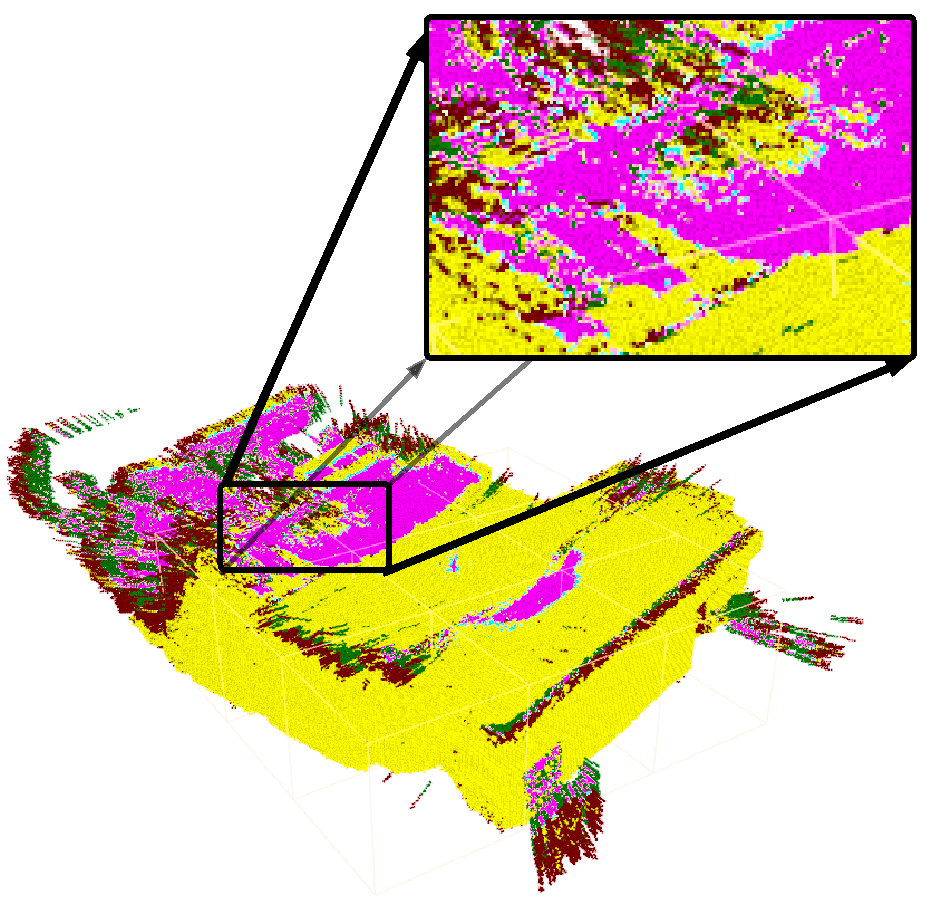
\includegraphics[width=.95\linewidth]{bresenham_zoom_p}
  		 \centering \caption{Assoziationen identifiziert mit Bresenham.}
  		 \label{fig:sp_bresenham}
	\end{subfigure}%
	\begin{subfigure}{.5\textwidth}
    	\centering
  		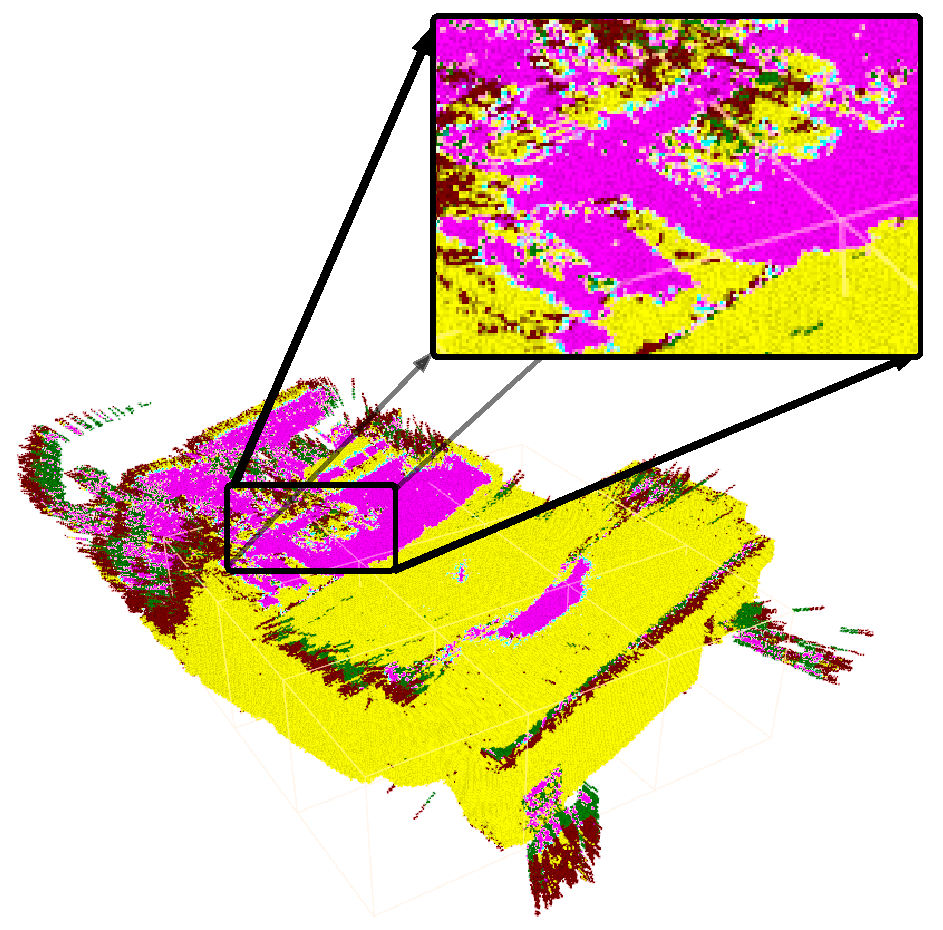
\includegraphics[width=.95\linewidth]{ray_tracer_zoom_p}
  		\centering \caption{Assoziationen identifiziert mit Ray-Tracing.}
  		\label{fig:sp_raytrace}
	\end{subfigure}
	\caption{Gegenüberstellung der generierten Assoziationen für einen Beispieldatensatz. Die durch Bresenham gefunden Assoziationen sind auf der linken Seite, die durch Ray-Tracing auf der rechten dargestellt. In diesem Fall wurden von Bresenham $91.74\%$ der Zellen assoziiert, während vom Ray-Tracing $91.97\%$ der Zellen assoziiert wurden. Zellen in gelb: assoziierte TSDF Zellen mit $value < 0$, Zellen in pink: assoziierte TSDF Zellen mit $value > 0$, Zellen in türkis: approximierter Nulldurchgang (Wechsel von positivem zu negativem Wert), Rest: nicht assoziierte Zellen. Zellen die nicht assoziiert werden, sind in diesem Fall größtenteils Teil von Verdeckungen oder Reflektionen des Laserscans und können als Outlier identifiziert werden. Für beide Abbildungen ist zur Darstellung der Unterschiede ein Ausschnitt vergrößert dargestellt. Es zeigt sich, dass die Konturen der ermittelten Assoziationen beim Ray-Tracing weniger verrauscht sind. Zusätzlich ist beim Bresenham-Ansatz ein größeres Grundrauschen zu beobachten. Die Änderungen sind allerdings nur Minimal und können aus diesem Grund an dieser Stelle vernachlässigt werden.}
	\label{fig:bresenham_vs_raytrace}
\end{figure}

\subsection{Evaluation}
\label{section:association_evaluation}

Dieser Abschnitt befasst sich mit den Problematiken bei der Bestimmung von Assoziationen zwischen einer gegebenen Trajektorie und einer bestehenden TSDF-Karte. Zusätzlich erfolgt im zweiten Teil eine Evaluation der Laufzeiten zwischen dem Bresenham Algorithmus und dem Ray-Tracing. 

Im vorigen Abschnitt wurde beschrieben, dass ein je nach Datensatz variabler Prozentsatz der Karte nicht durch den Raytracer und ebenfalls nicht durch Bresenham mit einer der Posen assoziiert werden kann. Dieses Problem wird sowohl durch die diskreten Schritte beim Raytracer, als auch durch eine unpassende Wahl der nächsten Zelle im 3-D Bresenham Algorithmus ausgelöst. Diese beiden Probleme sorgen allerdings nur zum Teil für die nicht assoziierten Zellen. Eine wesentliche Ursache sind durch die Diskretisierung eintretende Verdeckungen und Reflexionen beziehungsweise nicht gefiltertes Sensorrauschen bei der Generation der Karte, das für einzelne in der Luft schwebende TSDF-Zellen sorgt. Ein Beispiel für beschriebene Verdeckungen sind zum Beispiel Türen. In der Realität kann ein Laserscanner beliebig nah am Türrahmen vorbei scannen. Hier wird der Sichtbereich durch die Tür lediglich vom Türrahmen eingeschränkt. In einer diskretisierten TSDF-Karte wird der Sichtbereich durch die Tür je nach der Auflösung der Karte eingeschränkt. Abbildung \ref{fig:Verdeckungen} zeigt dieses Problem schematisch in 2-D anhand einer Pose und einem Hindernis, wie zum Beispiel einem Pfeiler. Es ist erkenntlich, dass ein Teil des ursprünglichen Sichtbereichs nun durch die diskretisierte TSDF-Karte verdeckt ist und alle Zellen, die sich im verdeckten Bereich hinter dem Hindernis nicht mehr assoziiert werden können. Dies ist die Hauptursache für beschriebene Probleme bei der Assoziationsbestimmung und kann ohne zusätzliche Informationen innerhalb der TSDF-Karte nicht gelöst werden. Eine Möglichkeit wäre, es dem Raytracer zu erlauben, durch Wände hindurch zu sehen, was allerdings dazu führen könnte, dass Zellen mit der Pose assoziiert werden, die nicht zu ihr gehören. Dies ist einer der Hauptgründe für eine grundlegende Veränderung der Herangehensweise an das in dieser Arbeit formulierte Problem. \ref{section:ass_lc} eruiert weitere Probleme dieses ersten Ansatzes.

\begin{figure}
		\centering
		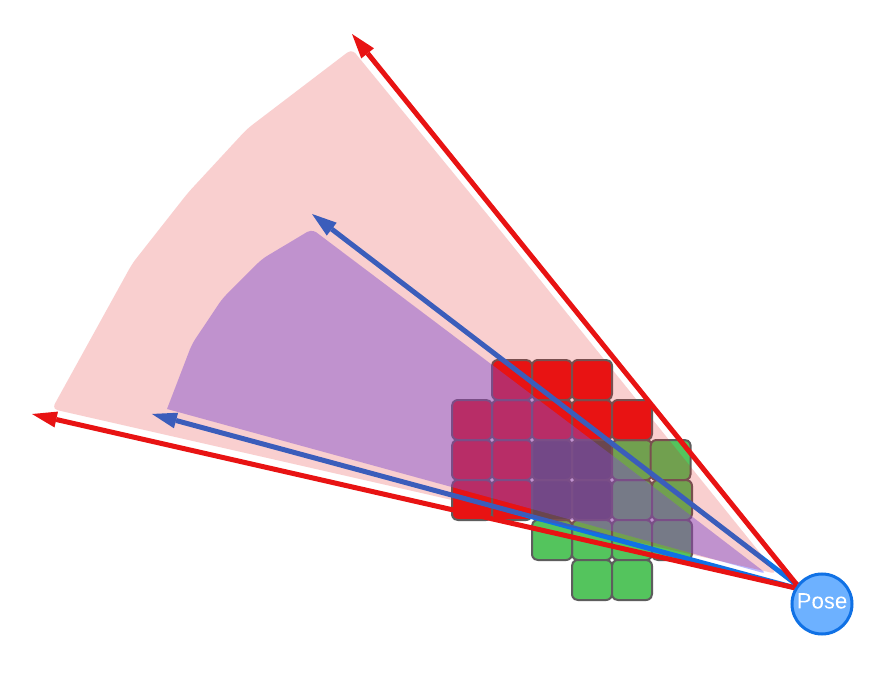
\includegraphics
			[scale=0.25]
			{Verdeckungen}
		\caption
			[Caption for LOF]{Diese Abbildung zeigt die Vergrößerung des Verdeckungsbereichs durch die Diskretisierung der Karte als TSDF. Zu sehen ist der ehemalige Verdeckungsbereich des in schwarz gefärbten Objektes. Dieser ist als halbtransparenter blauer Bereich gekennzeichnet. Darum herum zeigt sich der neue Verdeckungsbereich, der durch die Diskretisierung der Karte auftritt, ausgehend von der aktuell betrachteten Pose. Er ist halbtransparent in rot dargestellt. Diese Vergrößerung kommt durch die Beschaffenheit der Karte zustande. Nur außerhalb der roten Pfeile, also außerhalb des Verdeckungsbereichs kann mit Sicherheit gesagt werden, dass der simulierte Strahl Freiraum passiert. Durch die Diskretisierung hat sich der Bereich, in dem ein Objekt sein könnte, vergrößert. Dies ist die Hauptursache für nicht assoziierbare Zellen.}		                                                                                                                                     
		\label{fig:Verdeckungen}
\end{figure}

Abbildung \ref{fig:BresenhamVsRayTracing} zeigte eine Gegenüberstellung der Laufzeiten des Bresenham-Algorithmus in 3D gegenüber des vorgestellten Ray-Tracing Ansatzes. Es wird deutlich, dass durch die Einführung des Bresenham Algorithmus eine deutliche Steigerung der Effizienz erzielt wird.

\begin{figure}
		\centering
		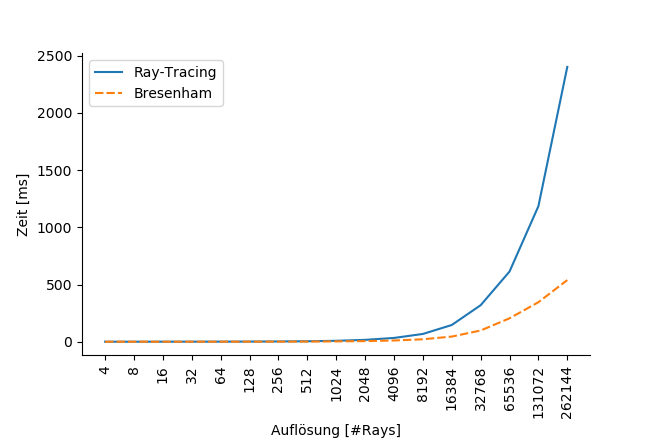
\includegraphics
			[scale=0.7]
			{BresenhamVsRayTracing}
		\caption
			[Caption for LOF]{Laufzeiten der vorgestellten Algorithmen zur Bestimmung der Assoziationen. Es handelt sich bei den jeweiligen Werte um das Mittel der Laufzeiten der Simulation mehrerer künstlicher Scans der beiden hier verglichenen Algorithmen, ausgehend von ungefähr 30 verschiedenen Positionen. Es ist zu sehen, dass -- obwohl der Zeitbedarf beider Algorithmen exponentiell mit der Anzahl an Strahlen steigt -- der Bresenham Algorithmus wesentlich effizienter ist. Bei den Laufzeiten handelt es sich um nicht parallelisierte Ansätze. Beide Varianten können durch die Nutzung einer \emph{Graphics Processing Unit (GPU)} zur Parallelisierung oder mittels CPU basierter Parallelisierung deutlich beschleunigt werden. Diese Beschleunigung liegt jedoch nicht im Fokus dieser Arbeit. Dieses Benchmark bestätigt die Hypothese, dass die Laufzeit durch die Ausnutzung der Diskretisierung erheblich verbessert wird. wobei ähnliche Ergebnisse erzielt werden können.}		                                                                                                                                     
		\label{fig:BresenhamVsRayTracing}
\end{figure}

Der folgende Absatz beschäftigt sich mit der Identifikation von Schleifenschlüssen innerhalb dieses ersten Ansatzes.


\section{Schleifenschlüsse in der Nachbearbeitung}
\label{section:ass_lc}

Zur Lösung des Schleifenschluss-Problems ist eine regelmäßig eine Aussage darüber zu treffen, ob ein Roboter oder Sensorsystems räumlich gesehen an derselben Pose oder in der Nähe der aktuellen Pose bereits gewesen ist. Dies lässt sich zum Beispiel über eine Distanzheuristik ermitteln. Alle Posen, deren euklidische Distanz zur aktuellen Pose geringer ist als eine festgelegte Schwelle sind Kandidaten für potentielle Schleifenschlüsse, die dann in den Pose-Graph, gegeben durch die Posen des Roboters und gegebenenfalls vorige Schleifenschlüsse, eingefügt werden können. Um zu bestimmten, ob einer der ermittelten Schleifenschluss-Kandidaten für einen Schleifenschluss in Frage kommt, muss die Umgebung jeder einzelnen in Frage kommenden Pose gegen die Umgebung der aktuellen Pose verglichen werden. Das Mittel der Wahl ist hier ein Scan-Matching Ansatz wie vorgeschlagen in \cite{lu1997globally,shan2020lio,borrmann2008globally}. Dieser Ansatz basiert allerdings auf räumlichen Punktdaten, die an dieser Stelle nicht vorhanden sind. Die Einzige Repräsentation der Umgebung ist die bereits fertiggestellte TSDF-Kartendarstellung. Aus dieser können allerdings Punktwolken approximiert werden. Grundlage dafür bildet in dieser Arbeit der zuvor entwickelte Raytracer. Dieser wird wie gehabt mit einer an den verwendeten Laserscanner angepassten Auflösung initialisiert und alle Strahlen werden schrittweise verlängert. Anstelle nun Assoziationen zu ermitteln, wird der erste Schnitt des Raytracers mit einem Nulldurchgang, einem Wechsel von positiven auf negative TSDF-Werte, gesucht. Ist ein solcher gefunden, wird die Ebene zwischen den beiden Voxeln berechnet, die die gesuchte Oberfläche am besten beschreibt. Diese Ebene ergibt sich aus den Positionen der Voxel $\vec{V_i}$ und $\vec{V_j}$, sowie den zugehörigen TSDF-Werten $v_i$ und $v_j$. Die TSDF-Werte bestimmen, wo die Ebene zwischen den beiden Voxeln liegt. Gegeben die Zentren der Voxel $\vec{c_i}$ und $\vec{c_j}$ in globalen Koordinaten, sowie die zugehörigen TSDF-Werte ist die Ebene beschrieben durch einen Ortsvektor $\vec{v_{ij}}$, sowie eine Normale $n_{ij}$. Die beiden Komponenten berechnen sich wie folgt:

\begin{myequation}
\vec{v_{ij}} = \vec{c_i} + \left(\vec{c_j} - \vec{c_i}\right) \cdot \frac{\abs{v_i}}{\abs{v_i}+ \abs{v_j}}
\end{myequation}

\begin{myequation}
\vec{n_{ij}} = \left(\vec{c_j} - \vec{c_i}\right)
\end{myequation}

Auf Basis der durch $\vec{v_{ij}}$ und $n_{ij}$ gegebenen Ebene lässt sich nun ein Punkt der Punktwolke als Schnitt des betrachteten Strahls mit der zuvor berechneten Ebene errechnen. Das Ergebnis dieser Approximation ist in Abbildung \ref{fig:pointcloud_approximation} dargestellt. Eine Zuordnung der approximierten Punktwolke zur Pose von welcher ausgehend die Punktwolke generiert wurde ist jedoch nicht sinnvoll, da unbekannt ist, welcher Teil der Karte tatsächlich von dieser Pose aus generiert wurde. Dasselbe Problem gilt auch für die Bestimmung von Punktwolken aus einer statischen Karte zur Berechnung potentieller Schleifenschlüsse um auf Basis der Schleifenschlüsse erneut die Karte zu optimieren. Dies scheitert schon bei der Generierung von Punktwolken aus einer potentiell unvollständigen oder gänzlich falschen Karte. Die approximierten Punktwolken stellen dann in jedem Fall auch unvollständige oder falsche Daten dar. Auch ein Scan-Matching mit potentiell unvollständigen oder falschen Daten ist nicht zielführend. Aus den genannten Gründen wird die Idee der Punktwolkenapproximation zur Identifikation von Schleifenschlüssen an dieser Stelle verworfen.

\begin{figure}
	\centering
	\begin{subfigure}{.5\textwidth}
 		 \centering
  		 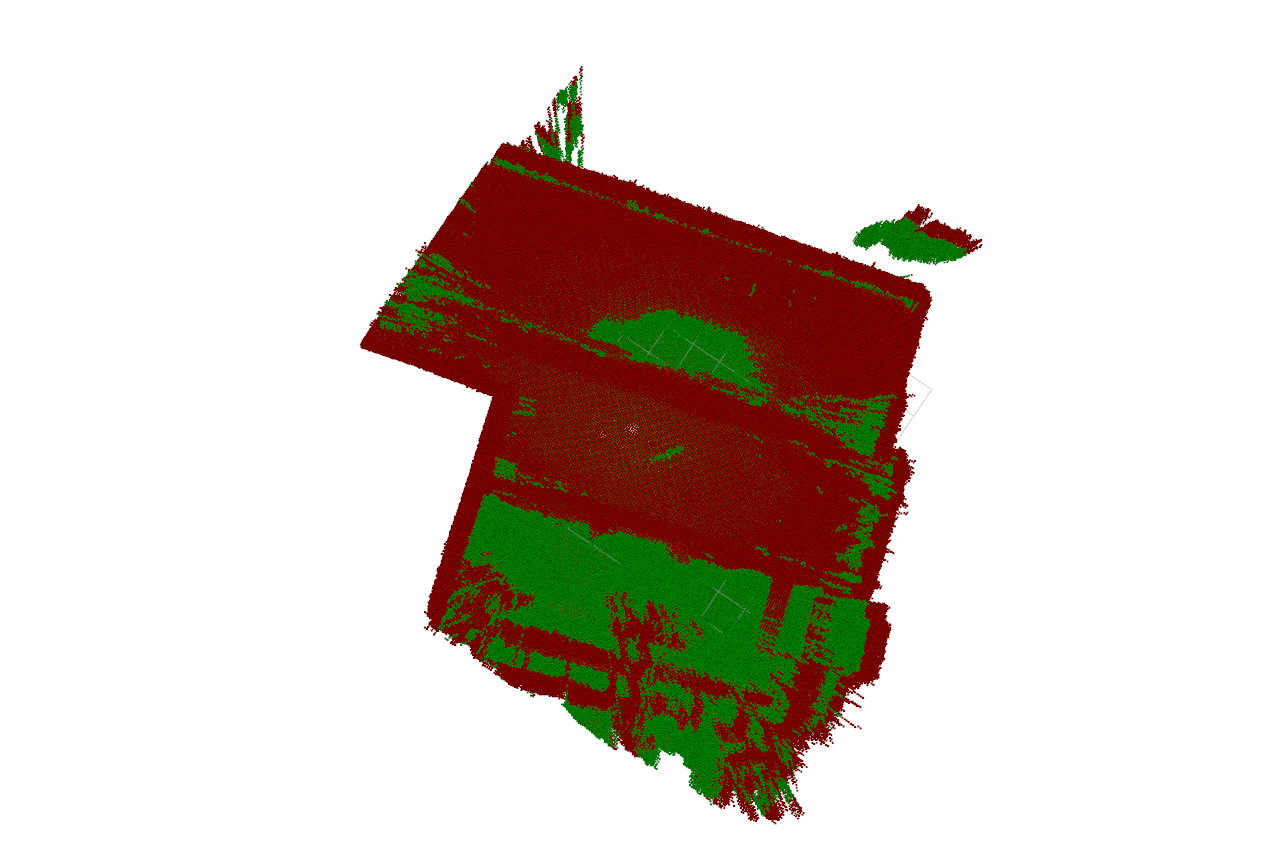
\includegraphics[width=1.15\linewidth]{single_tsdf}
  		 \centering \caption{Lokale TSDF Karte ausgehend von einer festgelegten Pose.}
  		 \label{fig:single_tsdf}
	\end{subfigure}%
	\begin{subfigure}{.5\textwidth}
    	\centering
  		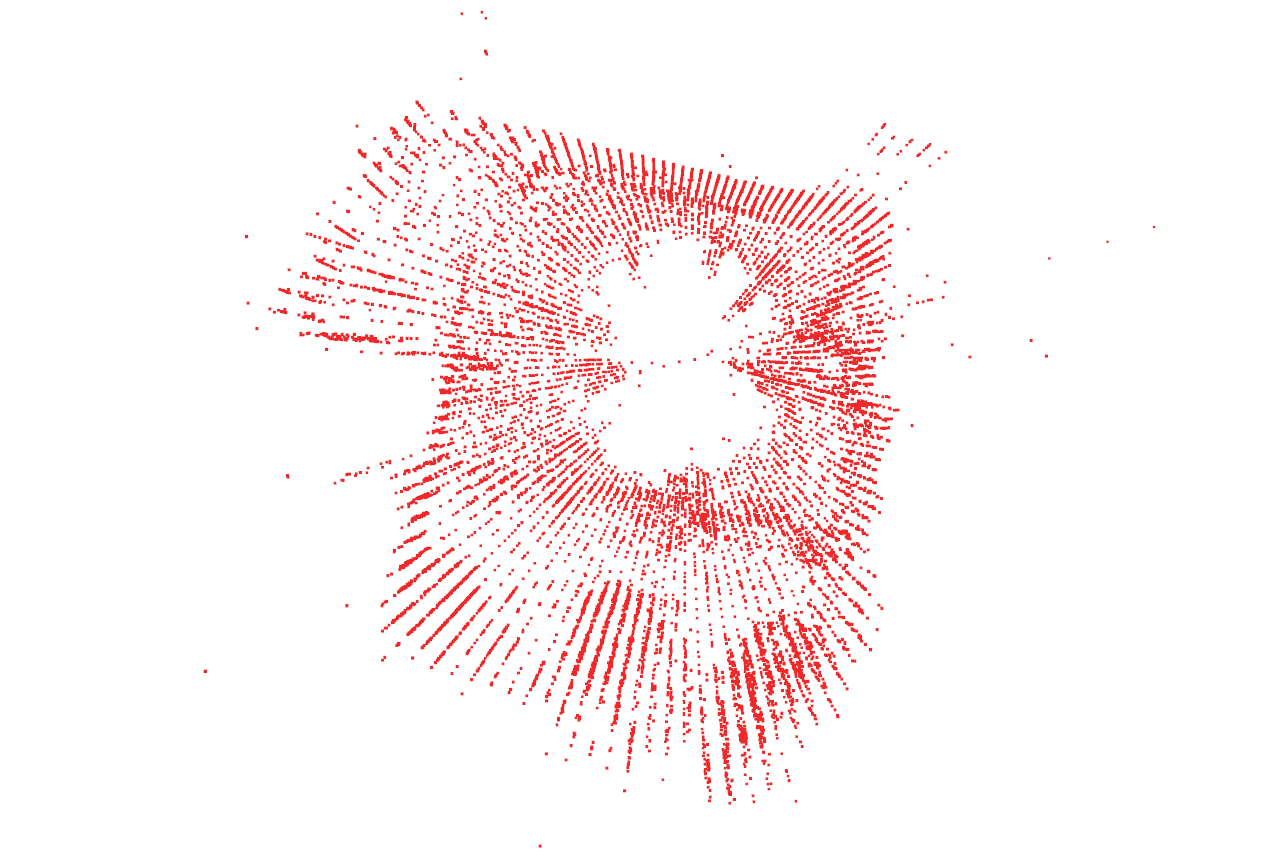
\includegraphics[width=1.15\linewidth]{approx_cloud}
  		\centering \caption{Aus der lokalen Karte generierte Punktwolke.}
  		\label{fig:approx_cloud}
	\end{subfigure}
	\caption{Gegenüberstellung eines Ausschnitts der TSDF-Karte und einer dazugehörigen, approximierten Punktwolke.}
	\label{fig:pointcloud_approximation}
\end{figure}

Im Folgenden wird unabhängig vom Ergebnis dieses Abschnitts, der die Problematik der Detektion von Schleifenschlüssen in der gegebenen Kartenrepräsentation darlegt, untersucht inwiefern ein Karten-Update auf Basis der generierten Assoziationen möglich ist.

 
\section{Karten-Update mittels generierter Assoziationen}

Dieser Abschnitt befasst sich mit dem Problem des TSDF-Kartenupdates, gegeben ein initialer Pfad $\mathfrak{P}_{init}$ und ein durch Schleifenschlüsse optimierter Pfad $\mathfrak{P}_{opt}$, sowie eine generierte Karte auf Basis des initialen Pfades. Ziel ist die Erstellung einer optimierten Karte, angepasst an den optimierten Pfad $\mathfrak{P}_{opt}$. Um dieses Ziel zu erreichen, müssen Teilbereiche der Karte entsprechend der Veränderungen der Posen verschoben werden. Dazu ist eine Assoziation zwischen Teilen der Karte und den zugehörigen Posen herzustellen. Entsprechend wurde ein Manager implementiert, der die zu bestimmenden Assoziationen verwaltet. Jeder Pose des alten Pfades wird ein HDF5-serialisierbares Assoziations-Objekt zugewiesen. Die Assoziationen selbst werden in einer \emph{1:N} Beziehung durch Ray-Tracing oder den vorgestellten 3-D-Bresenham Ansatz generiert. Dies liefert für jede Position $P_{i} \in \mathfrak{P}_{init}$ eine Menge $M = \left\lbrace C_1, ..., C_N \right\rbrace$, wobei die Anzahl der Assoziationen für jede Position unterschiedlich ist.

Die grundsätzliche entwickelte Logik für das Update der Karte auf Basis der generierten Assoziationen wird im Folgenden diskutiert. Zunächst wird in einem ersten Schritt für jedes Pose-Paar aus initialem und korrigiertem Pfad eine Pose-Differenz errechnet. Diese wird später genutzt um die neue Position assoziierter Zellen zu bestimmen. Gegeben die initialen Posen aus Pfad $\mathfrak{P}_{init}$, sowie die optimierten Posen aus $\mathfrak{P}_{opt}$, berechnen sich die einzelnen Pose-Differenzen beziehungsweise Transformationen $T_i$ wie folgt:

\begin{myequation}
T_i = \left(T_{i \rightarrow map}^{opt}\right)^{-1} \cdot T_{i \rightarrow map}^{init}
\end{myequation}

Im Anschluss daran werden drei Level von Daten generiert, die jeweils aufeinander aufbauen und den Informationsgehalt erhöhen. Zwei dieser Level verwenden Hashmaps um schnell detektieren zu können ob ein Eintrag für eine Zellposition schon existiert um dann entsprechend reagieren zu können. \emph{Level-1} enthält für jede assoziierte TSDF-Zelle ein Tupel der alten Zellposition, der neuen, akkumulierten Zellposition, des zugehörigen TSDF-Werts und Gewichts, sowie einen Zähler für die Anzahl an Posen, die mit dieser Zelle assoziiert werden. Gegeben ein Array der mit der aktuellen Zelle $\vec{C_i}$ assoziierten Posen $\left[P_x, ..., P_{x+n}\right]$, sowie ein Array aus Pose-Differenzen, gegeben als Transformationsmatrix, $\left[T_0, ..., T_{N-1}\right]$ berechnet sich die akkumulierte Zellposition dabei wie folgt:

\begin{myequation}
\vec{C_{acc}} = \sum_{j = x}^{x+n} T_j \cdot \vec{C_i}
\end{myequation}

Anhand der generierten \emph{Level-1} Daten lassen sich nun \emph{Level-2} Daten generieren. Hier wird berücksichtigt, dass die neue Position mehrerer initialer TSDF-Zellen identisch sein kann. In diesem Fall wird hier zunächst das arithmetische Mittel der TSDF-Werte und Gewichte gebildet und der neuen Position zugewiesen. Da für die Akkumulation dieser Daten Hashmaps verwendet wurden, haben die nun generierten Daten keinerlei räumliche Zusammengehörigkeit. Dies führt zu Problemen, wenn sich die zu schreibende Zelle außerhalb der aktuellen lokalen Karte befindet und diese entsprechend verschoben werden muss. Das Verschieben der Karte ist eine Ressourcen und zeitintensive Operation, die möglichst selten ausgeführt werden sollte. Durch die Unordnung muss im schlimmsten Fall für jede neue Zelle eine Verschiebung beziehungsweise ein \emph{Shift} stattfinden. Bei Millionen von TSDF-Zellen und einer durchschnittlichen Dauer des Shifts von über einer Sekunde, würde alleine dieser Schritt über $10$ Tage in Anspruch nehmen. Dementsprechend sind \emph{Level-3} Daten spezifisch angeordnet, um die Anzahl an Shifts auf ein Minimum zu reduzieren. Dazu wird die \emph{3-D Bounding-Box} des Raumes berechnet, den die neuen Zellpositionen einnehmen. Durch eine Aufteilung der Bounding-Box in Quader der Größe der lokalen Karte und eine Zuordnung der Zellen zu jedem dieser Quader wird die Anzahl der Shifts auf das gesuchte Minimum reduziert und die benötigte Zeit von Tagen auf Sekunden reduziert. Schlussendlich werden die initialen, assoziierten Zellen gelöscht und die neuen Zellpositionen mit den berechneten TSDF-Werten und Gewichten in die Karte geschrieben. Alle nicht assoziierbaren Zellen werden gelöscht. Da allerdings in der Regel kein globales, sondern nur ein lokales Update der TSDF-Karte vorgenommen werden soll lässt sich durch eine lokale Assoziationsbestimmung nicht sagen, ob die nicht assoziierbaren Zellen bedenkenlos gelöscht werden können, weil sie gegebenenfalls in einer globalen Assoziationsbestimmung assoziiert werden könnten. Ohne sicherzustellen, dass dies nicht der Fall ist, riskiert ein Löschen der genannten Zellen einen nicht zu kompensierenden Informationsverlust, was die Idee eines lokalen Updates in diesem Falle zunichte macht.

Wie in vorigen Abschnitten herausgestellt ist, kann zusätzlich nicht mit Sicherheit gesagt werden, dass jede so assoziierte Zelle auch von der assoziierten Pose generiert wurde. Dies lässt sich anhand von Abbildung \ref{fig:Assoziationsprobleme} zeigen. Durch einen Fehler in der Registrierung im initialen Pfad befindet sich eine Pose an einer fehlerhaften Stelle. Von dieser Pose aus wurde allerdings bereits ein -- ebenfalls fehlerhaftes -- TSDF Update durchgeführt. Die Daten, die zu dieser Pose gehören befinden sich nun hinter einer Wand, die zuvor von anderen Posen aus erstellt wurde. An dieser Stelle kann nun unmöglich ermittelt werden, welche Pose für die Erstellung der fehlerhaften Wand verantwortlich ist. Da der implementierte Raytracer nicht durch Wände hindurch schauen kann, wird daher ein falscher Teilbereich der Karte mit dieser fehlerhaften Pose assoziiert. Das Problem doppelter Wände ist dabei ein Problem, dass durch akkumulierten Drift im SLAM regelmäßig auftritt und durch Schleifenschlüsse gelöst werden kann. Dazu müssen die fehlerhaften Daten, wie zum Beispiel fehlerhaft positionierte Wände, allerdings auch mit den entsprechenden Posen assoziiert werden können. Diese Prämisse kann mit diesem Ansatz nicht erfüllt werden. 

\begin{figure}
		\centering
		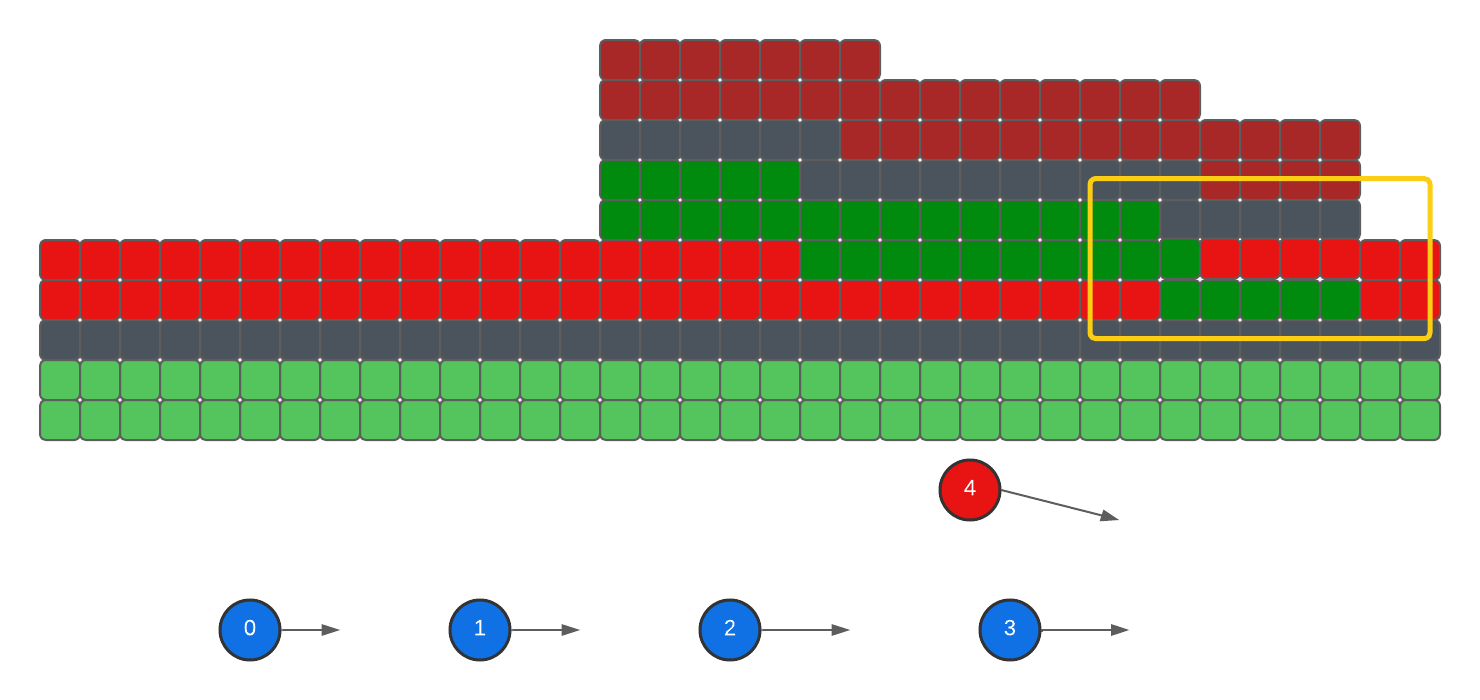
\includegraphics
			[scale=0.25]
			{Assoziationsprobleme}
		\caption
			[Caption for LOF]{TSDF-Karte nach Update durch eine fehlerhaft registrierte Pose (Pose 4, dargestellt in rot). Der fehlerhaft hinzugefügte Teil der TSDF-Karte ist farblich durch einen dunkleren Rot- und Grünton hervorgehoben. Eine Assoziationsbestimmung ausgehend von Pose 4 würde hier nicht den fehlerhaften Teil der Karte assoziieren da dieser hinter einer Wand befindlich ist. Der stattdessen mit dieser Pose assoziierte Teil der Karte wurde ursprünglich von anderen Positionen aus generiert. Der gelbe Rahmen markiert einen Teil der Karte, indem bereits generierte TSDF-Zellen mit den Werten neu erstellter Zellen verrechnet werden müssen. Der neue TSDF-Wert errechnet sich dann gemäß der alten, sowie neuen Gewichte und Werte. Ein mögliches Szenario dieses Updates für den Fall, dass die Gewichte beider Zellen jeweils $1$ ist, ist in der Abbildung dargestellt. Es wird deutlich, dass die TSDF-Karte durch die fehlerhaften Daten nun eine Inkonsistenz in den Gradienten aufweist, die nicht ohne Weiteres aufgelöst werden kann. Die Farben der Zellen im Überlappungsbereich wurde auf Basis der Zelle gewählt, die dominiert, also den größeren Einfluss auf das Endergebnis hat.}		                                                                                                                                     
		\label{fig:Assoziationsprobleme}
\end{figure}

Zusätzlich zum oben beschriebenen Problem existiert ein weiteres Problem, dass die Zellennachbarschaften betrifft. Benachbarte Zellen einer Wand sollten auch in der korrigierten Variante in direkter Nachbarschaft liegen, sodass die lokale Konsistenz der Karte gewährt bleibt. Wird nun eine Zelle von zwei verschiedenen Pose assoziiert und auf Basis eines Mittels der Pose-Änderungen verschoben, die Nachbarzelle allerdings durch einen Diskretisierungsfehler nur von einer Pose aus assoziiert und entsprechend verschoben, werden die beiden Zellen auseinander gezogen. Dies sorgt für ein merkliches Rauschen in der Karte und für zusätzliche Ungenauigkeiten. Eine Lösung hier wäre die lokale Konnektivität der Karte beim Update zu berücksichtigen. Dies wurde im Rahmen dieser Arbeit, besonders aufgrund der oben genannten Probleme allerdings nicht weiter verfolgt.

Um den oben beschriebenen Update-Prozess zu evaluieren, wurden einfach Transformationen, wie eine gleichmäßige Translation oder Rotation des Pfades vorgenommen und ein Kartenupdate auf Basis dieses neuen Pfades durchgeführt. Gleichmäßige Translationen stellten in dieser Hinsicht mit Ausnahme der nicht assoziierbaren Zellen keine Probleme dar. Sobald der Pfad oder Teile des Pfades in eine beliebige Richtung rotiert werden, trifft dies nicht mehr zu und durch die beschriebenen Probleme verliert die Karte ihre lokale Konnektivität und es bleibt lediglich ein inkonsistentes Rauschen. Fast jeglicher räumlicher Informationsgehalt geht verloren.

Der nachfolgende Abschnitt evaluiert die um jetzigen Zeitpunkt gefundenen Erkenntnisse und beschreibt, wie im weiteren Verlauf der Arbeit vorgegangen wird.


\section{Evaluation und Zusammenfassung}

Ziel dieses Kapitels ist die die Evaluation des Ansatzes zur Optimierung eines gegebenen Pfades durch Schleifenschlüssen und -- damit verbunden -- eine Optimierung der initial gegebenen TSDF-Karte auf Basis der zugrunde liegenden Pose-Änderungen. Die vorigen Absätze haben gezeigt, dass in grundlegenden Fällen, wie gleichmäßigen Translationen, ein Update mit dem vorgestellten Ansatz möglich ist. Diese grundlegende Fälle sind allerdings eine Abstraktion, die im realen Fall nicht gegeben ist. Zusätzlich scheitert der Ansatz bereits an der Ermittlung des optimierten Pfades. Wie oben beschrieben ist das Auffinden von Schleifenschlüssen und damit verbunden eine Optimierung des Pfades basierend auf den gegebenen Daten nicht möglich. Zudem gibt es mehrere Probleme bei der Ermittlung der Assoziationen, wie vergrößerte Verdeckungsbereiche durch die Diskretisierung der TSDF-Karte oder gänzlich falsch eingetragene Teilbereiche der Karte, die wiederum von anderen Teilen der Karte verdeckt und entsprechend nicht mehr assoziiert werden können. Aufgrund der Fülle der genannten Probleme und dem Nichtvorhandensein von Lösungen wird nun an dieser Stelle der erste Ansatz verworfen. Stattdessen wird im Folgenden auf einer größeren Datenbasis gearbeitet, die auch die Nutzung aufgenommener Punktwolken erlaubt. Dies ermöglicht eine Nutzung dieses Ansatzes sowohl innerhalb eines vorhandenen SLAM Ansatzes, als auch losgelöst in einem Nachbearbeitungsschritt. Ziel ist die Untersuchung von Schleifenschlüssen, sowie globalen und partiellen Updates der TSDF-Karte auf Basis dieser erweiterten Datenbasis. Das folgende Kapitel widmet sich nun der Grundlage für die Optimierung der Karte, der Identifikation von Schleifenschlüssen und damit verbunden der Optimierung der Roboter-Trajektorie beziehungsweise des Pfades.


